% last updated in April 2002 by Antje Endemann
% Based on CVPR 07 and LNCS, with modifications by DAF, AZ and elle, 2008 and AA, 2010, and CC, 2011

\documentclass[runningheads]{llncs}
\usepackage{graphicx}
\usepackage{amsmath,amssymb} % define this before the line numbering.
\usepackage{ruler}
\usepackage{color}
\usepackage[width=122mm,left=12mm,paperwidth=146mm,height=193mm,top=12mm,paperheight=217mm]{geometry}

%added by Mohammad
\usepackage{amsmath}
\usepackage{graphicx}
\usepackage{epsfig}
\usepackage{amsmath}
\usepackage{amssymb}
\usepackage{algorithmic}
\usepackage{algorithm}
\usepackage{enumerate}
\usepackage{subfigure}
\usepackage{wrapfig}
\usepackage{upgreek}
\begin{document}
% \renewcommand\thelinenumber{\color[rgb]{0.2,0.5,0.8}\normalfont\sffamily\scriptsize\arabic{linenumber}\color[rgb]{0,0,0}}
% \renewcommand\makeLineNumber {\hss\thelinenumber\ \hspace{6mm} \rlap{\hskip\textwidth\ \hspace{6.5mm}\thelinenumber}}
% \linenumbers
\pagestyle{headings}
\mainmatter
\def\ECCV12SubNumber{***}  % Insert your submission number here

\title{Ground Level To Aerial Image Matching Dataset And Benchmark} % Replace with your title

\titlerunning{ECCV-12 submission ID \ECCV12SubNumber}

\authorrunning{ECCV-12 submission ID \ECCV12SubNumber}

\author{Anonymous ECCV submission}
\institute{Paper ID \ECCV12SubNumber}

\maketitle

\begin{abstract}

% what's GLAID
% what's the purpose of GLAID
% what's the new challenge of GLAID
% how do we assess the existed methods for the new challenge
% what's the impact and result

Ground Level to Aerial Image Dataset (GLAID) is a challenging image dataset for image based geolocation.  It was created to enable the study of matching ground level images to $45^\circ$ aerial images, which has not been studied by the popular datasets that focus on matching images within the same condition.  The new challenges of cross condition matching include wide disparities in viewpoint and imaging conditions which often lead to feature matching failure.  To assess the strength and weakness of the existed methods, we benchmark top-down holistic image-as-texture based matching and bottom-up local interest point near-duplicate retrieval, providing an overview of the performance for the new challenge.  Finally, by analyzing the failure case for the existed approaches, we help to identify the future research directions for cross condition image geolocation.

\end{abstract}

% motivation/ goal/ related works
\section{Introduction}

\label{sec:intro}

% ==================First Paragraph================================== 
% Current approach is driven by existed dataset

% IM2GPS Hays08								Hays08
% Tiny Image									Torralba08
% Mapping the World's Photo		Crandall09  Flickr
% SUN attribute								Xiao10
% Location recognition using prioritized feature matching								Li2010				Cornell dataset

% City-Scale Location Recognition																				Schindler07
% Accurate Image Localization Based on Google Maps Street View					RoshanZamir10

Image based geolocation draws the attention from computer vision society in the past few years.  The massive collections of publicly available imagery is the key to enable location recognition.  \cite{Hays08}, \cite{Torralba08}, \cite{Li10}, \cite{Crandall09}, \cite{Xiao10}, \cite{Li10} harvest millions of geotagged images from photo sharing website.  \cite{Schindler07}, \cite{RoshanZamir10} also collect millions of images from the street view services along tens to hundreds kilometer of the street side.  With the large image database, the exciting progress has been made by applying popular object recognition techniques at two ends of the spectrum: holistic image-as-texture based matching (e.g., “the photo depicts an Iberian scene”) and local interest point based near-duplicate retrieval for famous landmarks (e.g., “the photo depicts the Sagrada Família”).  One common property shared by the both methods is that the query image should be taken \emph{within-condition} as the images in database for successful retrieval.

%1. image based geolocation draws attention from Computer Vision society in past few years.
%2. The key reason to enable the proliferation of field is the large image data set
%3. Variety of public available geotagged images on the Internet. photo sharing websites, Google Street View services
%4. The exciting progress has been made by the method inspired by previous data with near duplicate image retreival method.  (popular landmark)
%5. One common property shared by the previous methods is that near duplicate approach can produce good result for matching image within the same condition.

% ==================Second Paragraph==================================
% Introduce the dataset: setting, why do we need this kind of techniques, challenge, expected result
% The hope and the future work of GLAID

On the contrary of the popularity of matching images from photo sharing websites and street view services, the $45^\circ$ aerial imagery receives less attention in the wave of data driven location recognition despite the aerial imagery database has the mertis of wide and uniform coverage of locations, easy availability, and accurate geotagged images.  The above metioned merits could potentially complement the existed databases which put more emphasis on matching popular landmarks or street images.  However, the mismatch of disparity of view and imaging conditions between the query image and image database might arise the new challengings for matching holistic features or finding the near-duplicate local descriptor.  Such \emph{cross-condition} image matching still mainly untouched and needs a systematic study to discover the performance limit with the existed methods.


%0. point out the aerial database receive less attention
%1. But aerial imagery has the advantages such as wide and uniform coverage, xxxx that could complement existed datasets.
%2. The new challenge the mismatch of disparity of view and imaging conditions could make near duplicate feature matching failure therefore making the problem extremely challenging
%3. It's unknown about how good the existed data driven approach can acheive when applying on GLAID


% ==================Third Paragraph==================================
We introduce GLAID that aims to match ground level image to $45^\circ$ aerial imagery database. We benchmark top-down holistic image-as-texture based matching and bottom-up local interest point near-duplicate retrieval, providing an overview of the performance for the new challenge.  We propose a new performance metric based on the ranking of correct location at the set of blockified aerial images.  We label the affine transoformation and point correspondences between of each query image to the aerial imagery database such that we can study the variation of the distance for the corresponded pair of local feature descriptors.  We hope that the experiment result of baseline benchmark can shed the light on the future research directions for ground level to aerial level mathcing or more general \emph{cross condition} image matching.
 
% 1. We introduce GLAID that aims to match query image to $45^\circ$ aerial imagery.
% 2. some feature of the dataset, the location and affine transformation
% 3. we benchmark the dataset
% 4. A new performance metric is introduced to genuine location.
% 5. we hope the experiement result can indentify the directions of research for cross condition matching

% ==================Fourth Paragraph==================================
This paper is organized as follow.  The next section reviews top-down and bottom-up approaches for geolocation in the related works.  Section \ref{sec:image} introduces the image collection and annotation of GLAID dataset.  The baseline experiment settings and the experiment result are shown in Section \ref{sec:experiment} and Section \ref{sec:result}.  Finally, we will analyze the common failure cases of the baseline approach and identify the future direction for cross condition ground level to aerial image matching.  

% Content and emphasis for each section
%1. in section 2, we discuss the two popular approches that are usually used for geolocation
%2. in section 3, we introduce the details of image dataset
%3. in section 4, we discuss the detail approach of our baseline experiment
%4. in section 4, we show the baseline experiment result
%5. in section 5, we discuss the failure case and the future work

%Local:
%Location Recognition using prioritized feature matching
%- P2F: set the number of uniquely matched feature to be N
%Accurate Image Localization Based on Google Maps Street View
%- voting
%City-Scale Location Recognition
%- vocabulary tree on SIFT

%The problem of geographically localizing an image presents a wide array of challenges in computer vision and machine learning.  To answer the question ``where was this photo taken?''~when GPS data is not available, one can appeal to a variety of publicly available geotagged images on the Internet, e.g., photo sharing websites, street view services, satellite and aerial imagery. The problem of matching and retrieving images captured \emph{within-condition} using nearest neighbor on semi-local descriptors is well studied.  The same problem is considerably more difficult for the case of cross-condition image matching, e.g., in which there are significant differences in the noise level, blur, or illumination between a given pair of images; see Fig.~\ref{dataset-b}. The mismatch of features can severely degrade the accuracy of nearest neighbor methods. A solution to the problem of cross-condition matching is therefore key to leveraging the vast and diverse array of geotagged image data available on the Internet.

%To address this problem, we propose a human-in-the-loop, active learning framework. We leverage the relative ease with which a human observer can establish correspondences between categorically similar local image regions corresponding to meaningful architectural or landscape primitives such as window pane, chimney or shrub. First, the user is asked to select a few distinctive regions of interest in the query (ground level) image. Then the user is asked to label some patches with similar or dissimilar appearance in the aerial image.  Given this data, we learn a metric space wherein the extracted features from the two images are directly comparable.  To reduce the human labeling effort and improve the accuracy of the computer vision method, the proposed system alternates between computer vision processing and requesting user feedback. During this process, the system intelligently selects the instances with highest expected information gain for labeling. This active learning framework iteratively improves the metric, thereby allowing the system to find the genuine location with reduced human effort.

%This paper is organized as follows. The next section reviews related work.  Section \ref{sec:hil} reviews the proposed human-in-the-loop system. Then the learning algorithm will be explained in Section \ref{sec:learning}. Sections \ref{sec:dataset}, \ref{sec:feature} and \ref{sec:exper} explain the GLAID dataset, feature extraction and matching, and experimental results respectively. Finally, we conclude in Section \ref{sec:concl}. 

\begin{figure}[t] 
\centering
\includegraphics[width=0.9\textwidth]{pictures/exampleImg} \label{example} }
\caption[]{Snapshot of GUI for relevance feedback from the user.}
\label{fig:exampleImg}
\end{figure}



% related work:
% introduce two approaches: holistic and local
\section{Related Works}

\label{sec:related_work}

% ==================First Paragraph================================== What drives the geolocation and go to where
% Current approach is driven by existed dataset
% IM2GPS dataset : performance, Mapping the World's photo, photo tourism
% build rome in one day type dataset : performance
% property shared among the dataset is: to get the accurate performance, the query and testing image should be within the similar condition
% still there are other resources on the internet which has the wide coverage but has not been discussed yet

% LOCAL DESCRIPTOR:
% build rome																														Agarwal09
% City-Scale Location Recognition																				Schindler07
% Detecting and Matching Repeated Patterns for Automatic Geo-tagging in Urban Environments	Schindler08
% From structure-from-motion point clouds to fast location recognition	Irschara09
% Location recognition using prioritized feature matching								Li2010				Cornell dataset
% Fast Image-Based Localization using Direct 2D-to-3D Matching					Sattler11
% Accurate Image Localization Based on Google Maps Street View					RoshanZamir10				Street View dataset
% Modeling and Recognition of Landmark Image Collections Using Iconic Scene Graphs		Li08


% HOLISTIC FEATURE:
% IM2GPS Hays08								Hays08
% Tiny Image									Torralba08
% Mapping the World's Photo		Crandall09
% SUN attribute								Xiao10

% Tour the World: building a web-scale landmark recognition engine	Zheng09

% Feature
% Modeling the shape of the scene: a holistic representation of the spatial envelope	Oliva01
% Lowe	Lowe99

% ==================Second Paragraph==================================
% Introduce the dataset: setting, why do we need this kind of techniques, expected result, challenge

% Geo-localization of street views with aerial image databases
% Related work 				Bansal11

% ==================Third Paragraph==================================
% The hope and the future work of GLAID

% ==================Third Paragraph==================================
% Content and emphasis for each section


Local:
Location Recognition using prioritized feature matching
- P2F: set the number of uniquely matched feature to be N
Accurate Image Localization Based on Google Maps Street View
- voting
City-Scale Location Recognition
- vocabulary tree on SIFT

%The problem of geographically localizing an image presents a wide array of challenges in computer vision and machine learning.  To answer the question ``where was this photo taken?''~when GPS data is not available, one can appeal to a variety of publicly available geotagged images on the Internet, e.g., photo sharing websites, street view services, satellite and aerial imagery. The problem of matching and retrieving images captured \emph{within-condition} using nearest neighbor on semi-local descriptors is well studied.  The same problem is considerably more difficult for the case of cross-condition image matching, e.g., in which there are significant differences in the noise level, blur, or illumination between a given pair of images; see Fig.~\ref{dataset-b}. The mismatch of features can severely degrade the accuracy of nearest neighbor methods. A solution to the problem of cross-condition matching is therefore key to leveraging the vast and diverse array of geotagged image data available on the Internet.

%To address this problem, we propose a human-in-the-loop, active learning framework. We leverage the relative ease with which a human observer can establish correspondences between categorically similar local image regions corresponding to meaningful architectural or landscape primitives such as window pane, chimney or shrub. First, the user is asked to select a few distinctive regions of interest in the query (ground level) image. Then the user is asked to label some patches with similar or dissimilar appearance in the aerial image.  Given this data, we learn a metric space wherein the extracted features from the two images are directly comparable.  To reduce the human labeling effort and improve the accuracy of the computer vision method, the proposed system alternates between computer vision processing and requesting user feedback. During this process, the system intelligently selects the instances with highest expected information gain for labeling. This active learning framework iteratively improves the metric, thereby allowing the system to find the genuine location with reduced human effort.

%This paper is organized as follows. The next section reviews related work.  Section \ref{sec:hil} reviews the proposed human-in-the-loop system. Then the learning algorithm will be explained in Section \ref{sec:learning}. Sections \ref{sec:dataset}, \ref{sec:feature} and \ref{sec:exper} explain the GLAID dataset, feature extraction and matching, and experimental results respectively. Finally, we conclude in Section \ref{sec:concl}. 




% dataset overview/ image collection method / ground truth definition
% residential image/ should I expand the dataset a little bit to cover different building variety?
% what annotation should I give
\section{Image Collection And Annotation}

\label{sec:image}

% ===================First Paragraph===============================
% how many query image; how many aerial images; where is the photo taken

% ===================Second Paragraph===============================
% the annotation: the scale and location of query image on the aerial map.  The point correspondence between two images

\begin{figure}[ht] 
\centering
\subfigure[{}]{ 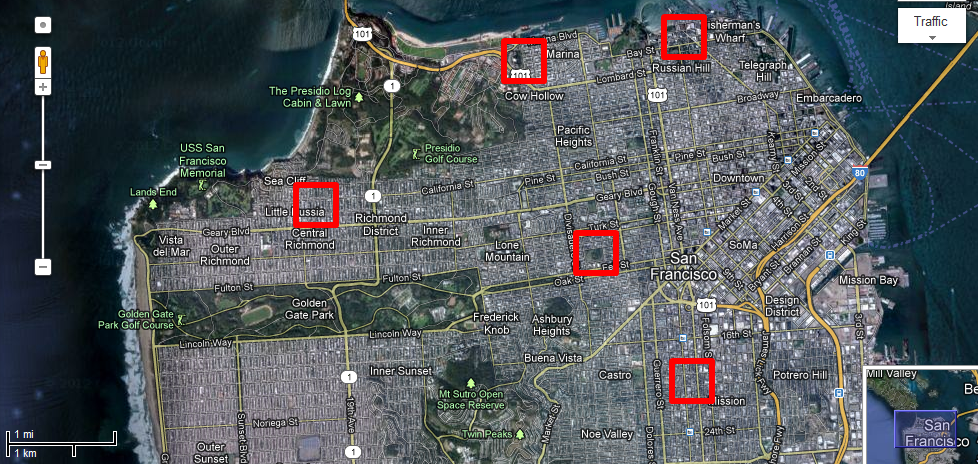
\includegraphics[width=0.4\textwidth]{pictures/collection-a} \label{collection-a} }
\subfigure[{}]{ 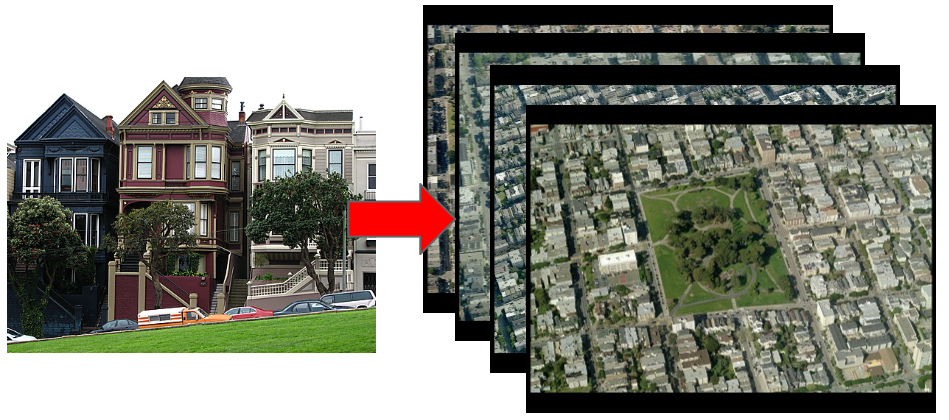
\includegraphics[width=0.4\textwidth]{pictures/collection-b} \label{collection-b} }
\caption[]{\subref{collection-a} We evaluate matching on the 5 areas bounded by red boxes. \subref{collection-b} Each query image matches to 4 aerial images in one area.}
\label{dataset}
\end{figure}


% performance metric
\section{Peformance Evaluation}

\label{sec:evaluation}

\begin{figure}[ht] 
\centering
\subfigure[{}]{ 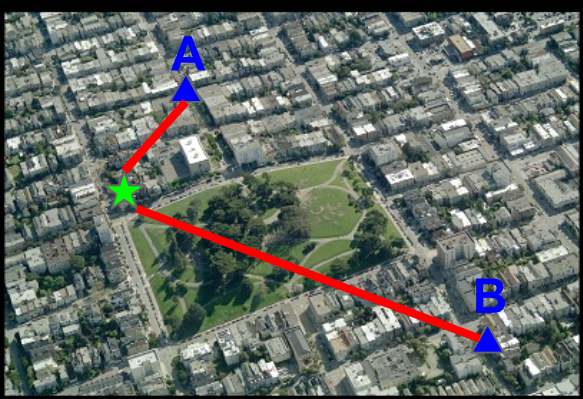
\includegraphics[width=0.3\textwidth]{pictures/eval-a} \label{eval-a} }
\subfigure[{}]{ 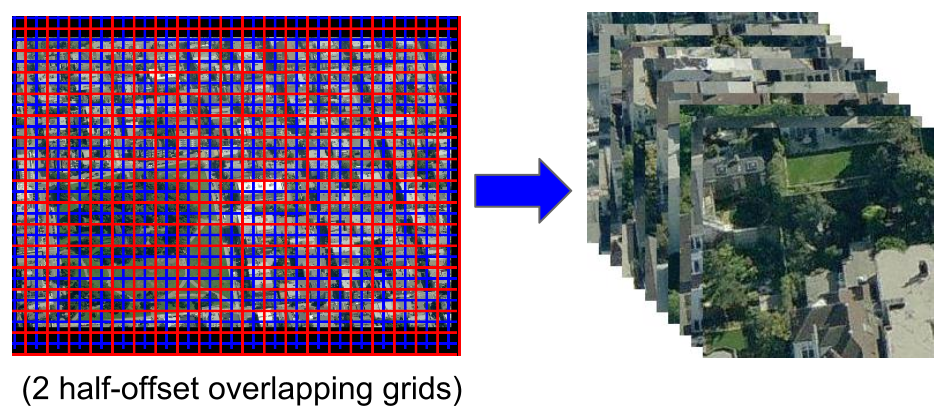
\includegraphics[width=0.5\textwidth]{pictures/eval-b} \label{eval-b} }
\caption[]{\subref{eval-a} Euclidean distance from a query (star) to a candidate location (A or B) is an unsatisfactory performance metric. \subref{eval-b} In our study we break the aerial views into blocks and use the rank of the true block as a performance metric.}
\label{eval}
\end{figure}


The evaluation on this dataset is done by first cutting the aerial image into overlapping blocks of size $200 \times 200$ pixels. Then the algorithm is asked to sort the blocks based on their matching scores. After that, the rank of the correct block is a used as a measure to compare different algorithms. Since the blocks are sorted based on matching score, it is desired for the correct block to have a low rank. We propose this measure because the traditional distance measures (e.g., Euclidean or geodesic) are not meaningful in this setting; see Fig.\ref{eval}\subref{eval-b}.  In the case of large search spaces, as in the IM2GPS setting, such a distance measure can reveal the neighborhoods in an entire country that have a similar visual texture to a query image.  In our setting, we only aim to find the genuine location such that user can verify the exact matched block. Therefore, we do not reward the matching if it misses the correct location but finds a non overlapping nearby location.

%we do not want to reward the matching algorithm if it misses the correct location but finds another location in the same city.

%The evaluation on this dataset is done by first cutting the aerial image into overlapping blocks of size $200 \times 200$ pixels. Then the algorithm is asked to sort the blocks based on their matching scores. After that, the rank of the correct block is a used as a measure to compare different algorithms. Since the blocks are sorted based on their matching scores, it is desired for the correct block to have a low rank. This measure is designed because the traditional distance measures are not meaningful for this purpose. For example, Euclidean spatial distance between the correct location and output of the algorithm is not a meaningful measure because if the algorithm does not discover the genuine location, it does not matter if the output is very far or rather close. This is true when the search is done within a small neighborhood, but if the search space was larger to cover different cities, finding the correct city is not far from being possible because of the correlation between the appearance of the buildings in the same city. Then in that case the spatial distance will be more meaningful. But in GLAID since there is no correlation between adjacent buildings, finding a wrong but close location should not be rewarded. This can be seen in Fig.\ref{eval}\subref{eval-b}, in which Point A is not preferred to B because of its shorter distance to the correct location. 
%[[I sense that this observation will be considered controversial by some reviewers, 
%  Mohammad: I changed the paragraph a little bit, it may be better. What do you think? Should we remove this observation?  Serge: yes, this is better.]]





%This dataset will be available for public use on UCSD Vision Group's Website \footnote{http://vision.ucsd.edu/}.
%This dataset will be available for public use on our group's website\footnote{link is removed for anonymity}.


% evaluation methodology: 1) distance; 2) block ranking 
\section{Baseline Experiments}

\label{sec:experiment}




% experiment on evaluation: 1) bottom up; (sift); 2) top down (gist)
% bottom up: interested point detection? + SIFT feature detection + SIFT feature/SSIM/xxxx
% top down: GIST matching for block processing (or hide the idea here first?)
\section{Result}

\begin{figure}[ht] 
\centering
\subfigure[{}]{ 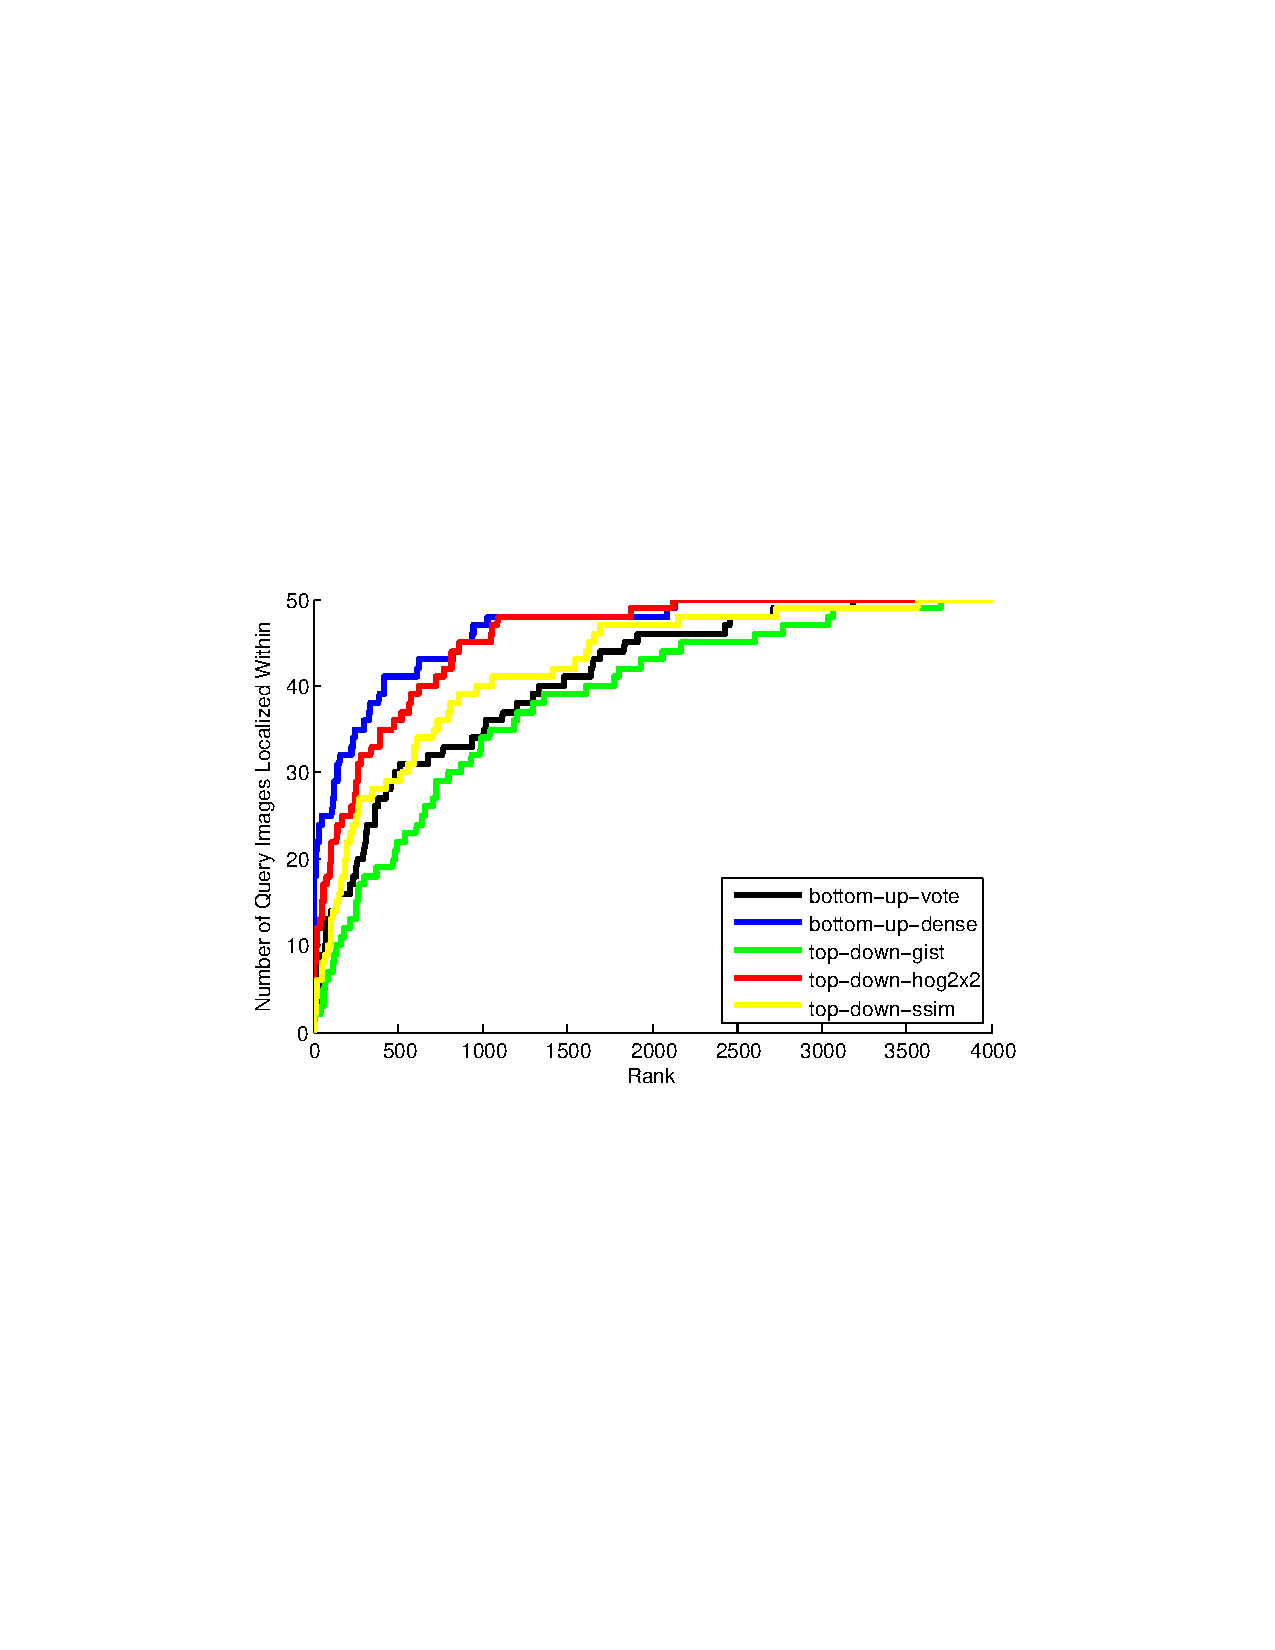
\includegraphics[width=0.5\textwidth]{pictures/result-a} \label{result-a} }
%\subfigure[{}]{ \includegraphics[width=2.5in]{pictures/result-b} \label{result-b} }
\caption[]{\subref{result-a} Example ground level query image and 4 associated aerial images. \subref{result-b} Highlighting the appearance difference in across the two imaging conditions.}
\label{result}
\end{figure}

\label{sec:result}




% wrap up
\section{Discussion And The Future Works}

\label{sec:discussion}




\bibliographystyle{plain}
\bibliography{ECCV_bib}

\end{document}
